%%%%%%%%%%%%%%%%%%%%%%%%%%%%%%%%%%%%%%%%%%%%%%%%%%%%%%%%%%%%%%%%%%%%%%%%%%%%%%%%
%2345678901234567890123456789012345678901234567890123456789012345678901234567890
%        1         2         3         4         5         6         7         8

\documentclass[letterpaper, 12 pt, conference]{ieeeconf}  % Comment this line out
                                                          % if you need a4paper
%\documentclass[a4paper, 12pt, conference]{ieeeconf}      % Use this line for a4
                                                          % paper

\IEEEoverridecommandlockouts                              % This command is only
                                                          % needed if you want to
                                                          % use the \thanks command
\overrideIEEEmargins
% See the \addtolength command later in the file to balance the column lengths
% on the last page of the document

\usepackage{hyperref}
\usepackage[utf8]{inputenc}
\usepackage{enumerate}
\usepackage{natbib}
\usepackage{graphicx}
\usepackage[spanish]{babel}
\hypersetup{
    colorlinks=true,
    linkcolor=blue,
    filecolor=magenta,      
    urlcolor=cyan,
}

% The following packages can be found on http:\\www.ctan.org
%\usepackage{graphics} % for pdf, bitmapped graphics files
%\usepackage{epsfig} % for postscript graphics files
%\usepackage{mathptmx} % assumes new font selection scheme installed
%\usepackage{times} % assumes new font selection scheme installed
%\usepackage{amsmath} % assumes amsmath package installed
%\usepackage{amssymb}  % assumes amsmath package installed

\title{\LARGE \bf
Práctica 5: circuitos de control de tiempo
}

%\author{ \parbox{3 in}{\centering Narshion Ngao*
%         \thanks{*Use the $\backslash$thanks command to put information here}\\
%         Msc. Computer Systems - 2018\\
%         Jomo Kenyatta University of Agriculture \& Technology \\
%       
%}}

\author{Universidad de San Carlos de Guatemala \\% <-this % stops a space
Escuela de Ciencias Físicas y Matemáticas\\
Laboratorio de Circuitos\\
Segundo Semestre 2019
}


\begin{document}



\maketitle
\thispagestyle{empty}
\pagestyle{empty}

\section{Objetivos}
\begin{itemize}
    \item General: estudiar circuitos básicos para el control de tiempo astable y monoestable.
    \item Específicos:
    \begin{enumerate}
    \item Experimentar con la constante de tiempo correspondiente a un circuito RC en corriente directa.
    \item Analizar la configuración astable del circuito integrado 555.
    \item Comparar las ventajas en el uso de dispositivos pasivos y activos para control de tiempo.
\end{enumerate}
\end{itemize}


\section{Materiales}
\begin{itemize}
    \item 1  capacitor electrolítico 3300 uF
    \item 1 resistencia 10K ohm 1/4W.
    \item 1 switch selector de dos posiciones.
    \item 1 teléfono con cámara o cámar digital.
    \item 2 multímetros.
    \item Alambres para protoboard de cualquier tipo (y pinzas para cortarlo, si es necesario).
    \item 1 fuente.
    \item 1 protoboard.
\end{itemize}
\pagebreak

\section{Diagramas}

\begin{figure}[h!]
    \centering
    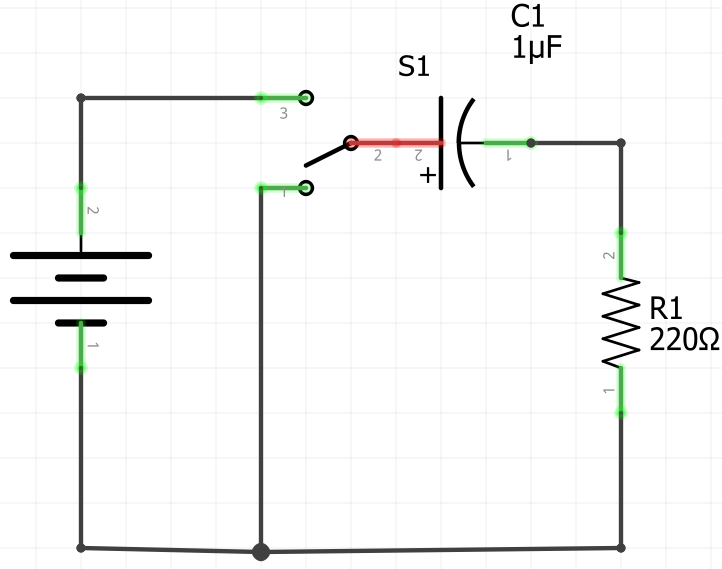
\includegraphics[scale=0.5]{C1.png}
    \caption{Esquema circuito RC para adquisición de datos.}
\end{figure}


\section{Procedimiento y reporte de resultados}
Seguir todos los pasos que a continuación se enlistan respondiendo en una hoja adicional lo que sea requerido de forma ORDENADA y CLARA.

\begin{enumerate}
    \item Armar en protoboard el circuito de dos mallas seleccionables por un switch de la Figura 1.
\begin{figure}[h!]
    \centering
    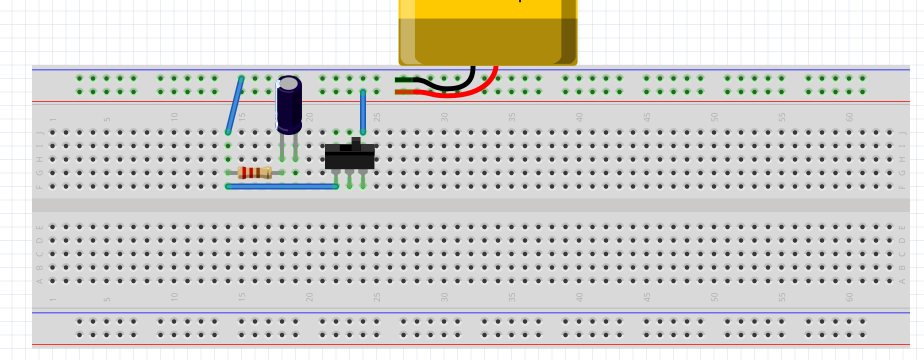
\includegraphics[scale=0.5]{B1.png}
    \caption{Circuito para adquisición de datos.}
\end{figure}
    
    \item Posicionar el selector en la malla RC sin voltaje.
    \item Posicionar voltímetro y amperímetro en lugares apropiados para medición.
    \item Comenzar a grabar video desde este momento para capturar los valores de los multímetros durante todo el procedimiento.
    \item Al tener todo listo, cambiar el selector hacia la otra posición para agregar una fuente de voltaje al circuito.
    \item Observar los cambios de voltaje y corriente en el circuito hasta notar que dejan el estado transitorio.
    \item Cambiar el selector a la posición inicial y seguir grabando los valores de los multímetros para obtener los valores de descarga del capacitor.
    \item Realizar tablas  con las mediciones de voltaje y corriente versus tiempo para cada etapa del circuito (carga y descarga). Tomar en cuenta las incertezas.
    \item Graficar los valores obtenidos en las tablas.
    \item Utilizando el software de preferencia y valores ideales, comparar las curvas del inciso anterior con las ideales. Evaluar su coincidencia.
    \item Calcular el valor ideal de $\tau$ para el circuito utilizado. ¿5$\tau$ corresponde a la cantidad de tiempo que tardó el circuito en alcanzar las asíntotas? ¿Varía el tiempo de carga y de descarga total?
    \item Realizar un reporte completo escrito en LaTex con formato IEEE para presentar resultados de la práctica. Las secciones mínimas requeridas son resumen, objetivos, introducción, marco teórico, diseño experimental, resultados, discusión de resultados y conclusiones.
    
    \item La sección de 555 será cubierta en taller de PCB. Incluir las conclusiones y recomendaciones en el reporte.

\end{enumerate}
\addtolength{\textheight}{-12cm}   % This command serves to balance the column lengths
                                  % on the last page of the document manually. It shortens
                                  % the textheight of the last page by a suitable amount.
                                  % This command does not take effect until the next page
                                  % so it should come on the page before the last. Make
                                  % sure that you do not shorten the textheight too much.

\end{document}